
\newgeometry{top=1cm, bottom=1cm, left=1cm, right=1cm,
               marginparsep=0cm, marginpar=0pt}
\newpage

\makeatletter
\cxset{bache scale/.store in = \scalebache@cx,
    bache left column width/.store in = \bacheleftcolumnwidth@cx,
    bache imagei/.store in = \bacheimagei@cx,
    bache imagei caption/.store in = \bacheimageicaption@cx,
    bache imageii/.store in = \bacheimageii@cx,
    bache imageii caption/.store in = \bacheimageiicaption@cx,
    bache left header/.store in = \bacheleftheader@cx,
    bache header/.store in = \bacheheader@cx}%
\cxset{bache scale = 1,
    bache left column width = {\dimexpr\textwidth-.4\textwidth\relax},
    bache left header =,
    bache imagei = {./images/bache-01.jpg},
    bache imagei caption ={\begin{multicols}{2}\lorem\lorem\end{multicols}},
    bache imageii = {./images/nudeback.jpg},
    bache imageii caption = {JULES BACHE},
    bache header = \scalebox{.97}{THE DEAN OF US NUDE-PAINTERS}
    }%
\newenvironment{bache}{%
\parindent0pt
\renewenvironment{leftcolumn}{%
   \minipage[t]{\bacheleftcolumnwidth@cx}%
   \leavevmode   
  }{\endminipage}\hspace*{0cm}%
 \renewenvironment{rightcolumn}{%
   \minipage[t][\textheight-45pt][t]{.37\textwidth}%
   \mbox{}%
  }{\endminipage}\hspace*{0cm}% 
\begin{minipage}[t][\textheight][t]{\scalebache@cx\textwidth}%
\resizebox{\textwidth}{!}{\Large\bfseries\sffamily JULES BACHE GIVES HIS \$20,000,000 ART COLLECTION TO NEW YORK}\par%
\begin{leftcolumn}%
\mbox{}^^A
\par\leavevmode\includegraphics[width=\linewidth]{\bacheimagei@cx}\par
\bacheimageicaption@cx%
\end{leftcolumn}\hfill%
\begin{rightcolumn}%
\mbox{}^^A
\intextsep0pt
\@afterindentfalse\parindent1em
\begin{wrapfigure}{l}{0pt}
 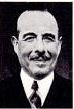
\includegraphics[width=.37\linewidth]{./images/bache-02.jpg}
\caption*{\bfseries\sffamily \bacheimageiicaption@cx}
  \end{wrapfigure}\ignorespaces
 }
{\end{rightcolumn}%
\end{minipage}%
} %
%

\begin{bache}
This layout has a dominant left column image. It is important to
ensure that the image has an aspect ratio to suit. Unfortunately
it is very difficult to crop and scale an image via \tex so a bit
of experimentation is appropriate.

It is also important to ensure that you add an adequate amount
of text during editing, otherwise the layout will not look very good. The right
column has two images (it really looks better when it has two images rather than
one and the bottom image is really a filler, if you have more or less
text you may have to go back and crop the image to suit. Any extra space on the right column is used as glue. The template also has a manual mode, where one can adjust the lengths and writing
a bit more accurately. \label{bache}

\vfill
\includegraphics[width=\linewidth]{../images/bache-03.jpg}
\end{bache}

\restoregeometry


\section{The bache template}
The bache template, named after the dominant photograph in the sample template
is an adaptation of a layout from a Life magazine. The basic layout is shown below and
a full page sample is shown on page~\pageref{bache}.

{\begin{center}

\cxset{bache scale=.7}
\fboxsep0pt
\resizebox{\scalebache@cx\textwidth}{!}{\begin{bache}
This layout has a dominant left column image. It is important to
ensure that the image has an aspect ratio to suit. Unfortunately
it is very difficult to crop and scale an image via \tex so a bit
of experimentation is appropriate.

It is also important to ensure that you add an adequate amount
of text during editing, otherwise the layout will not look very good. The right
column has two images (it really looks better when it has two images rather than
one and the bottom image is really a filler

\includegraphics[width=\linewidth]{./images/bache-03.jpg}
\end{bache}}

\end{center}
}

\begin{lstlisting}
\cxset{bache scale = 1,
    bache left column width = {\dimexpr\textwidth-.4\textwidth\relax},
    bache left header =,
    bache imagei = bache-01,
    bache imagei caption ={\begin{multicols}{2}\lorem\lorem\end{multicols}},
    bache imageii = nudeback,
    bache imageii caption = {JULES BACHE},
    bache header = \scalebox{.97}{THE DEAN OF US NUDE-PAINTERS}
    }%
\end{lstlisting}

Keeping simplicity in mind, we only require the user to fill the above template and to type only
a short piece of code and the text. It is preferable to write the last piece of
text, rather than insert this type of writing in the template, as one may need to iterate a 
couple of times to get the right amount of text.
\begin{lstlisting}
\begin{bache}
    text body on right column.
\end{bache}
\end{lstlisting}

I believe that filling a few lines of information in a template and then a short environment, is
the simplest way possible. A more complicated way is to set the template on manual and
build it piece by piece with commands.





\restoregeometry